%---A LaTeX template for Mechatronics ME 495 Capstone report.
\documentclass[twocolumn]{article}
\oddsidemargin=-0.35in
\topmargin=-0.75in
\headsep=0.1667in
\columnsep=0.25in
\textwidth=7.25in
\textheight=9.125in
\headheight=12pt

\usepackage{myfontstyle}			% Palatino & Euler fonts
\usepackage{graphicx}               % begin standard LaTeX macros
\usepackage{fancyhdr}               % fancy headers, see fancyhdr.pdf
\usepackage{fancyvrb}               % fancy verbatim environment, see fancyvrb.pdf
\usepackage{lastpage}               % used in the footer to specify the last page
\usepackage{amsmath}                % for log-like symbols
\usepackage{color}
\usepackage{dtklogos}
\newcommand{\bra}[1]{\langle #1|}
\newcommand{\ket}[1]{|#1\rangle}
\newcommand{\braket}[2]{\langle #1|#2\rangle} 

\begin{document}	%  <--- Here is where the document starts

\title{
	\vspace{-0.5in}\rule{\textwidth}{1pt}
	\begin{tabular}{ll}\begin{minipage}{4.75in}\vspace{6px}
			\noindent\Large Department of Mechanical Engineering\\
			\vspace{-12px}\\
			\noindent\large University of Washington\qquad 
		\end{minipage}&\begin{minipage}{2in}\vspace{6px}\small
		Stevens Way, Box 352600\\
		Seattle, WA 98195 USA\\
		206-543-5090
	\end{minipage}\end{tabular}
	\rule{\textwidth}{1pt}\vspace{0.25in}
	\Large
	Mechanical Impedance Control
}

\date{Mechatronics Capstone Design Report --- June 10, 2016}

\author{
	{Richard S Chen}\\
	rchen3@uw.edu
	\and 
	{Nathan Robert Dabling}\\
	ndabling@uw.edu
	\and
	{Fangzhong Guo}\\
	fzguo@uw.edu
	\and
	{James Kurniawan}\\
	kurnij@uw.edu
	\and
	{Kyle R Spangenberg}\\
	spangkyl@uw.edu
}

\maketitle


%---Executive Summary
\subsection*{Executive Summary{{\color{red}\ *}}}

This capstone project investigates the design and implementation of a variable-impedance controller. The basis for the control scheme is a set of functional specifications for the system to achieve. These requirements dictate the controller design as well as the motor and amplifier used. The controller is designed to compare the velocity of the actual system with a reference velocity that is calculated from the desired mass, spring, and damping.  The system, in this case, is a one-dimensional prototype consisting of a cart driven by a motor and belt 

Here is a suggested outline for Mechatronics ME 495 reports. Since the projects of all groups are different, feel free to modify the organization of this format to meet your project requirements. However, note that some sections ({\color{red}\bf{*}}) are required. 

%---Introduction
\subsection*{Introduction}

\noindent --Problem definition. \par
The main goal of this project is to demonstrate the viability of a variable impedance controller with the use of a one-dimensional prototype. Variable impedance control utilizes user input in order to achieve a desired state of mobility. The system senses a force and responds by changing its impedance to match the desired input parameters of the user. The user will be able to control the virtual weight, damping, and spring force. These virtual parameters will dictate how the system performs while being used. \par
There are many applications for this research and while only a simple prototype, the implications are far-reaching. With variable impedance control, a heavy object can feel lighter and be easier to maneuver. Lighter objects that don't provide enough feedback for a human can have their apparent weight increased. When human control and reasoning is desired over robot logic, variable impedance control can make a difference. This report goes over the preliminary research and modeling completed in order to fully realize a finished prototype in the near future.

\noindent --Functional requirements \par
<<<<<<< HEAD
At the beginning of the design phase, we set target values for the settling time and percent overshoot, found in \ref{specs}.
\begin{table}[H]
	\centering
	\caption{Functional Specifications}
	\label{specs}
	\begin{tabular}{|l|l|}
		\hline
		Target Requirement &          \\ \hline
		\%OS               & 5\%      \\ \hline
		Settling Time      & 0.15 sec \\ \hline
	\end{tabular}
\end{table}
 Using the targets, an appropriate motor and amplifier were attained. In selecting a motor, a reference had to be used to run simulations, so a motor with a torque constant of .11 N/m was used in tandem with an amplifier with a gain of .79 A/V. Using these sample motor and amplifier constants in the model, simulations were run through Simulink to verify that such a motor and amplifier combination would suffice by checking the maximum current, voltage, torque and rpm required against what the motor and amp could supply. Cases with low mass and damping proved to have the highest torque and current requirements because the velocity profile of such a system would involve very high accelerations. From the results we decided that damping must always be included in the reference system to limit the necessary torque. \par
After the design was finalized a functional specification map was created to guide the user's inputs. The motivation for this was observing that the low mass, low damping case performed reasonably well as long as the force input was small. In addition, a greater force could be applied if either the damping or mass was increased. This led to the conclusion that the limitations on the reference system parameters were actually coupled. Considering the restrictions that either increasing the mass or the damping would put on the acceleration of the reference system for a given force input, this conclusion seemed logical. To create the mapping, a calculation was done on the transfer function relating the force input to the required motor current.\begin{equation}
=======
At the beginning of the design phase, target functional specifications were set. The specifications were based on ambitious but attainable goals for percent overshoot and settling time. Using the targets, the motor and amplifier were sized. In selecting a motor, a reference had to be used to run simulations, so a motor with torque constant of .11 N/m was used in tandem with an amplifier with a gain of .79 A/V. Using these sample motor and amplifier constants in the model, simulations were run through Simulink to verify that such a motor amplifier combination would suffice by checking the maximum current, voltage, torque and rpm required against what the motor and amp could supply. Cases with low mass and damping proved to have the highest torque and current requirements because the velocity profile of such a system would involve very high accelerations. From the results it was decided that damping must always be included in the reference system to limit the necessary torque.
\begin{figure*}[th!]
	\centering
	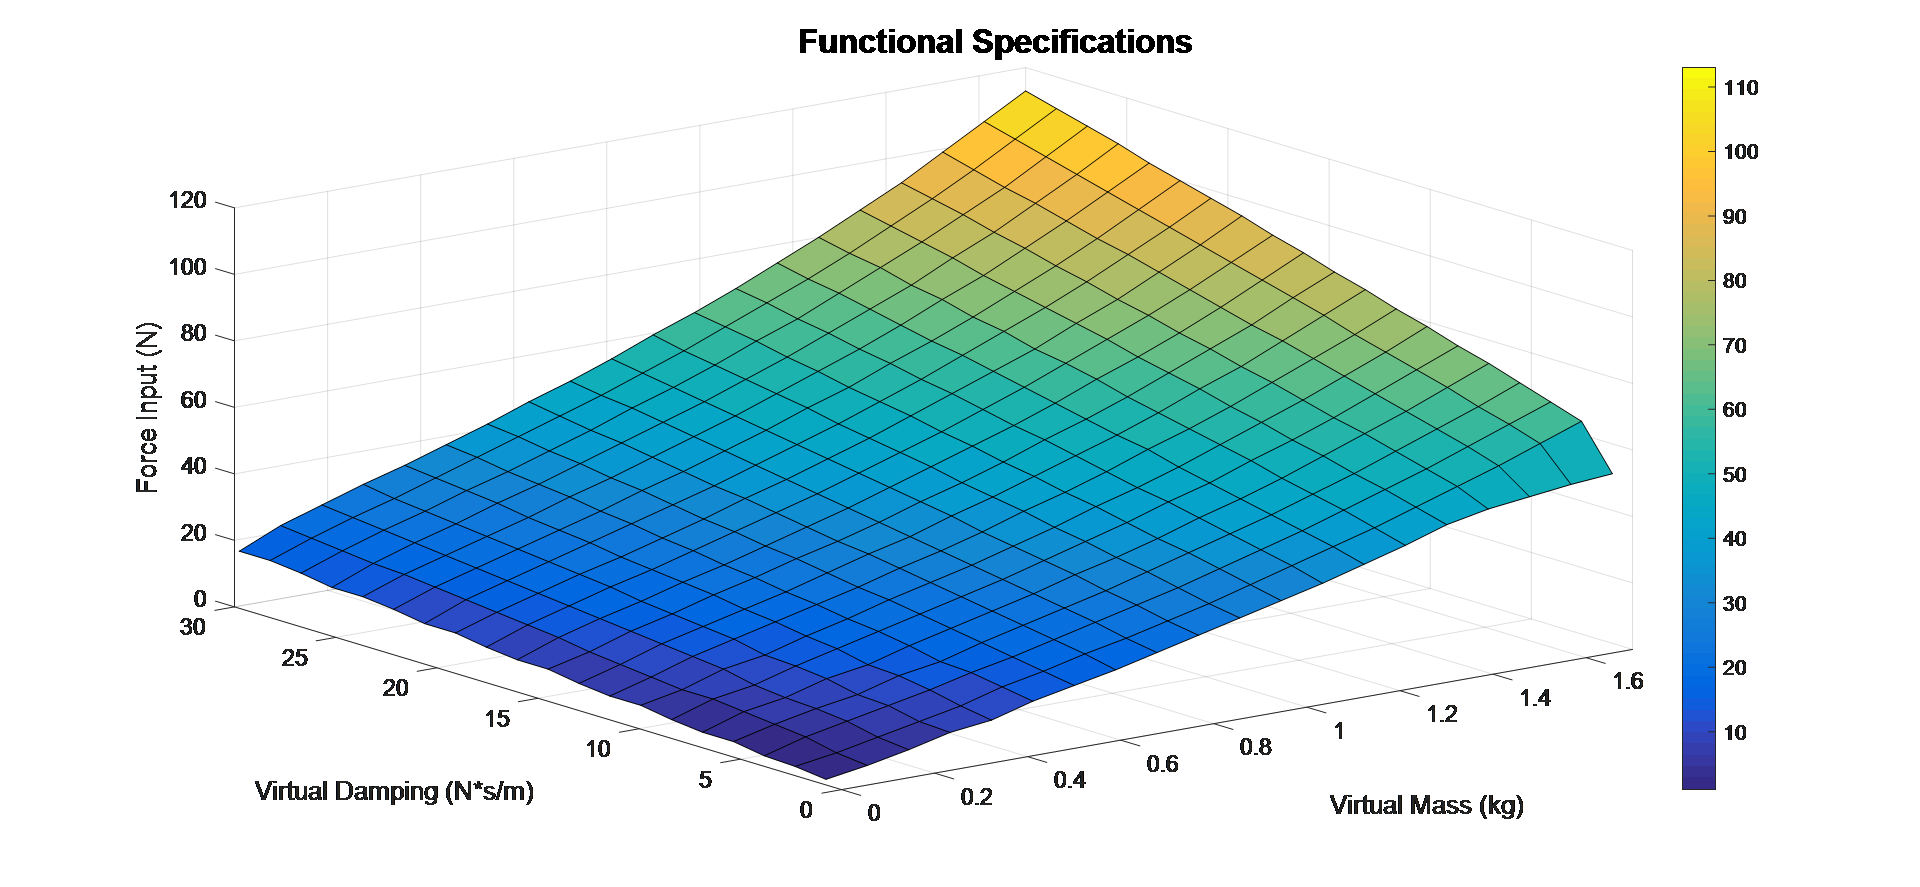
\includegraphics[width=1\linewidth]{Images/Functional_Specifications_Mapping}
	\caption{3D mapping of the maximum human input force for varying virtual mass and damping. Virtual stiffness is set to 5 N/m}
	\label{fig:Functional_Specifications_Mapping}
\end{figure*}
\newline \indent After the design was finalized a functional specification mapping was developed to guide the user's inputs. The motivation for this was observing that the low mass, low damping case performed reasonably well as long as the force input was small. In addition, a greater force could be applied if either the damping or mass was increased. This led to the conclusion that the limitations on the reference system parameters were actually coupled. Considering the restrictions that either increasing the mass or the damping would put on the acceleration of the reference system for a given force input, this conclusion seemed logical. To create the mapping, the transfer function relating the force input to the required motor current was calculated.\begin{equation}
>>>>>>> master
I = \frac{[K_{P}s+K_{I}][(\epsilon-M)s^{2}-Bs-K]}{[\frac{\epsilon}{K_{A}}s^{2}+\frac{K_{P}K_{M}}{r}s+\frac{K_{I}K_{M}N}{r}][Ms^{2}+Bs+K]}F
\end{equation}
Where 
\begin{equation}
\epsilon = M+\frac{JN^{2}}{r^{2}}
\end{equation}
\newline \indent The transfer function depends on the parameters of both the reference and actual systems, as predicted, but not in any clearly identifiable way. The mapping was generated numerically using successive approximation to determine what applied force would result in the current requirement exceeding the limitations of the amplifier, about 4.8 A. The parameters varied were the mass and damping, as the relationship between the spring and acceleration was less complex and more intuitive and the input force was a critical component of any mapping.
\newline \indent The mapping shown in Figure 1 is just a small portion of the effective range. This portion was selected because it demonstrates the very small force that can be applied when the reference system has very low mass. The maximum value of force shown is near 111 N which is approximately the limit of the load cell range. Theoretically, the force possible to apply would continue to increase beyond this point but the load cell would not read it as a greater force, so the system cannot handle greater forces regardless. If the load cell range was not the limiting factor, it is presumed that the force would increase with the damping and mass until the torque required to prevent the acceleration of the real system going beyond the reference system's response for the input force. In this way, the lower range of the the functional specification mapping can be seen as dependent on the ability of the motor to increase the acceleration of the real system and the higher range of the functional specification mapping can be seen as dependent on the ability of the motor to decrease the acceleration of the real system.


%---The Design
\subsection*{The Design}

\subsubsection*{ ---Description}
\subsubsection*{ ---Analysis}
Based on the design described in previous sections, a Simulink model of the closed loop system is created. The block diagram is similar to the control loop in 'Variable Impedance Based Human Machine Control for Docking of Manufacturing Fixtures'\cite{toni}. Shown in Figure \ref{fig:ControlLoop}, the model is split into four subsystems: Human Input, Reference System, Motor and Cart Plant. The simulation is based on a continuous control scheme. It first calculates the reference speed based on human input calculate the error between reference speed and actual speed. The error is then used as the input for PI controller to calculate the required power output that drives the motor plant.

\begin{figure*}[ht]
\centering
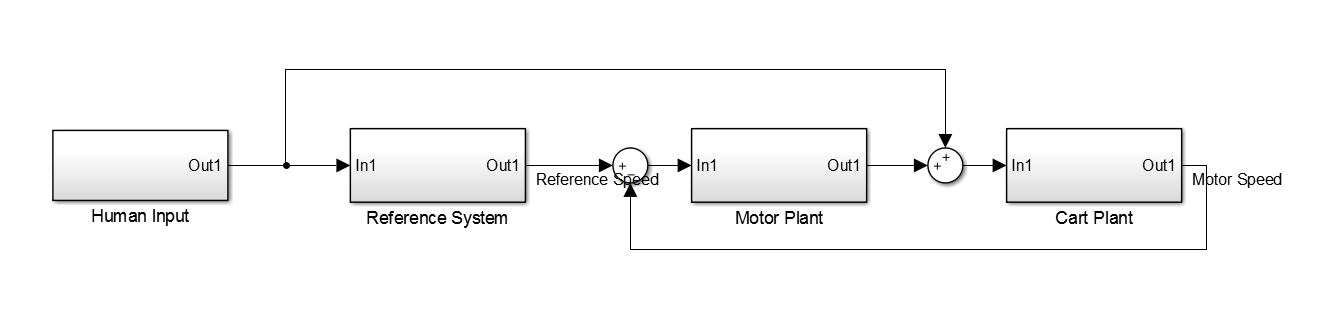
\includegraphics[width=1\linewidth]{Images/ControlLoop}
\caption{Block diagram of the impedance controller. Consists of human input; a reference system with mass, spring and damping parameters from user input; a motor plant and a modeled cart plant}
\label{fig:ControlLoop}
\end{figure*}

Human input for the model has three modes of inputs. Mode 0 is a standard step input with specified amplitude from user input. Mode 1 is a impulse input which has the same amplitude as mode 0, however it has a user defined impulse time. Mode 2 reads experimental data collected from the load cell, it is only used for performance analysis.

The reference system depicts the reaction of a mass-spring-damper setup to a specified input force. A illustrative graph for it is shown in Figure \ref{MSB}. In our model, it is assumed that the spring is always relaxed at the mass's initial position. It also assumes the system has no friction. It will simulate the mass's acceleration, velocity and position based on human input. The simulated speed is then used as reference for the closed loop control system.

\begin{figure}[h]
	\centering
	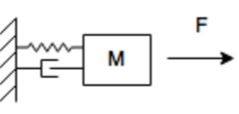
\includegraphics[width=0.5\linewidth]{Images/MSB}
	\caption{Reference System}
	\label{MSB}
\end{figure}

The motor and cart plants are models based on the actual components. Motor plant utilizes a PI controller designed for the system to calculate a control voltage from difference between reference and actual cart speed. The control voltage is then transformed into force applied on the cart through a series of amplifiers and mechanical translations. The cart plant will then calculate the actual speed using both human input force and motor force.

The simulation is used to determine the current, torque and speed requirement for the motor. After running boundary cases from the functional specification map, the peak current and torque requests are found to be no larger than 5A and 2.1N*m respectively, whereas continuous current and torque requests are no larger than 0.6A and 0.2N*m respectively. Samples of simulation results are included in Appendix {{\color{red}\ *}}.

Capability of the PI controller is also found through simulation. A set target speed is used to substitute reference velocity. By running a step response of the system, overshoot of the controller is found to be 18.9\%, whereas the settling time is found to be 0.12s.
\subsubsection*{ --- Mechanical} 
After completing the dynamic modeling and simulation, the mechanical design was next. The physical model consists of a track, motor, and the designed cart which simulates the object being moved. To secure the track, stabilizers for the motor and endcap were 3D printed and clamped to the table. The motor drives a V-Slot belt connected to the designed cart on a gantry plate that slides along the track. An isometric view of the CAD design (Figure \ref{fig:Isometric_Full_View}) and actual model (Figure \ref{fig:Iso_Real_Full}) are shown below.

\begin{figure}[H]
	\centering
	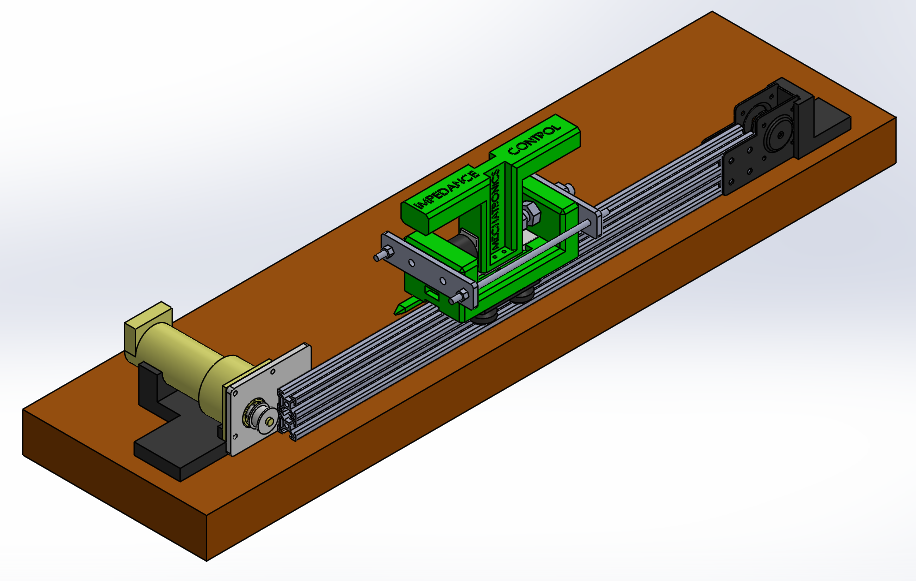
\includegraphics[width=1\columnwidth]{Images/Isometric_Full_View}
	\caption{Isometric CAD Model}
	\label{fig:Isometric_Full_View}
\end{figure}

\begin{figure}[H]
	\begin{center}
		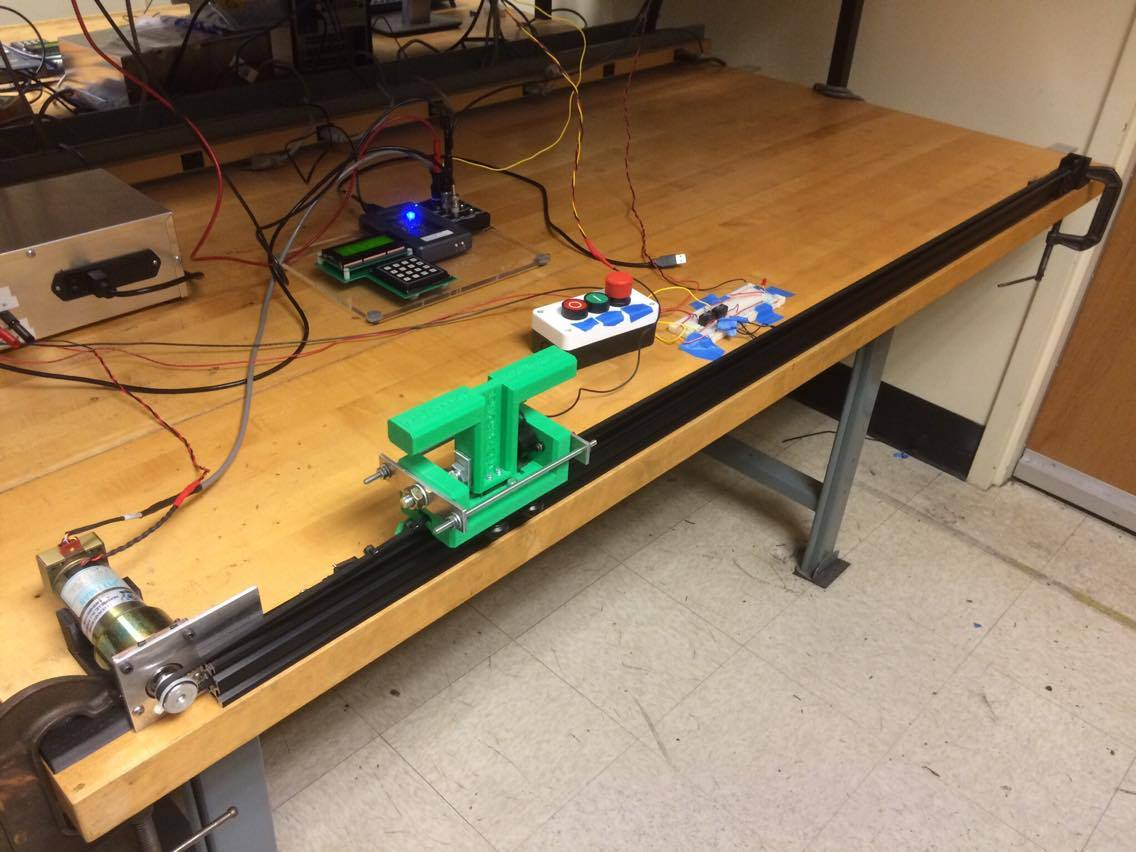
\includegraphics[width=1\columnwidth]{Images/Iso_Real_Full}
		\caption{Actual Prototype}
		\label{fig:Iso_Real_Full}
	\end{center}
\end{figure}

On the cart, there is a handle which is preloaded by an M10 Bolt onto a button load cell. Limit stops were hot glued to the bottom of the cart to hit the limit switches at the ends of the track which would turn off the system if anything went wrong. The cart, handle, and limit stops were 3D printed. The user will apply a force to the handle sensed by the load cell which will be the input for our computer model and the cart should move accordingly based on the reference model. The challenge is to ensure that the force from the user is all transmitted to the load cell for an accurate input to the system model. One can imagine that as the handle is preloaded, there will more friction to overcome.

The first step to tackle this problem is to use small aluminum connecting plates on both sides of the handle that contact the load cell and M10 preload bolt. Since the handle was 3D printed PLA, the pressure from small contacting point of the load cell and the M10 bolt would only deform the soft PLA material. Adding the aluminum connecting plates allows for a stiffer area of contact and a consistent force to be applied to the load cell.

\begin{figure}[H]
	\centering
	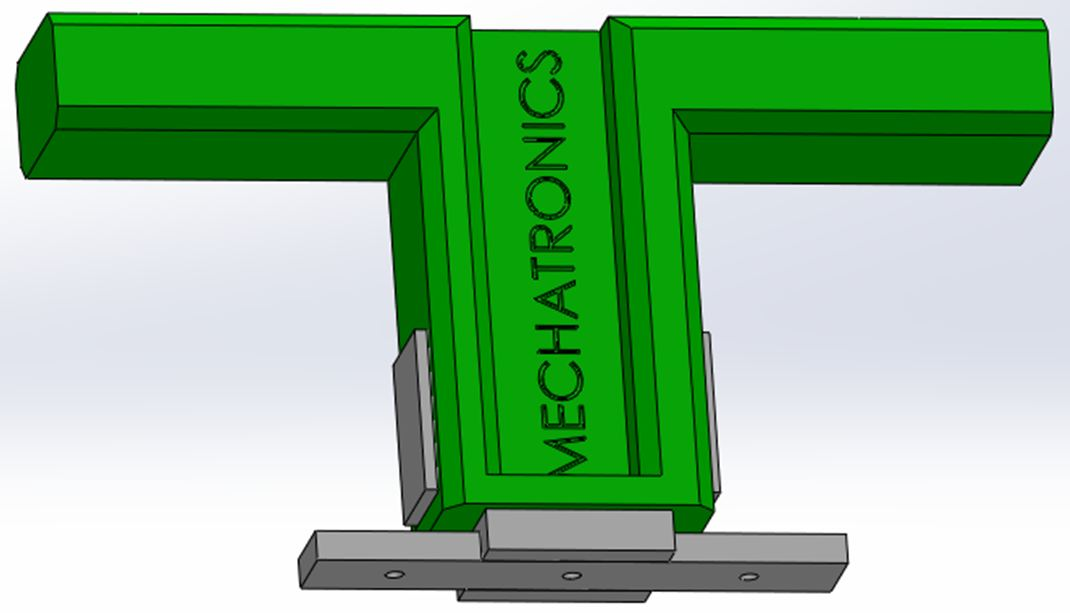
\includegraphics[width=1\columnwidth]{Images/Recirculating_Ball_Track}
	\caption{Handle on Recirculating Ball Track}
	\label{fig:Recirculating_Ball_Track}
\end{figure}

Taking a closer look, the handle is screwed on to a recirculating ball track as shown in Figure \ref{fig:Recirculating_Ball_Track}. The recirculating ball track is a key component to the mechanical design. Since the slider moves purely in a linear motion along the track, it minimizes friction and ensures that any force, even a torque, applied to the handle is completely transmitted to the load cell. Figure \ref{fig:Ball_Track_Cross_Section} shows a cross section of the handle and how it connects to the load cell, M10 preload bolt, ball track, and the rest of the cart. A labeled figure of the entire system is shown in Figure \ref{fig:Annotated_Front}.

\begin{figure}[H]
\centering
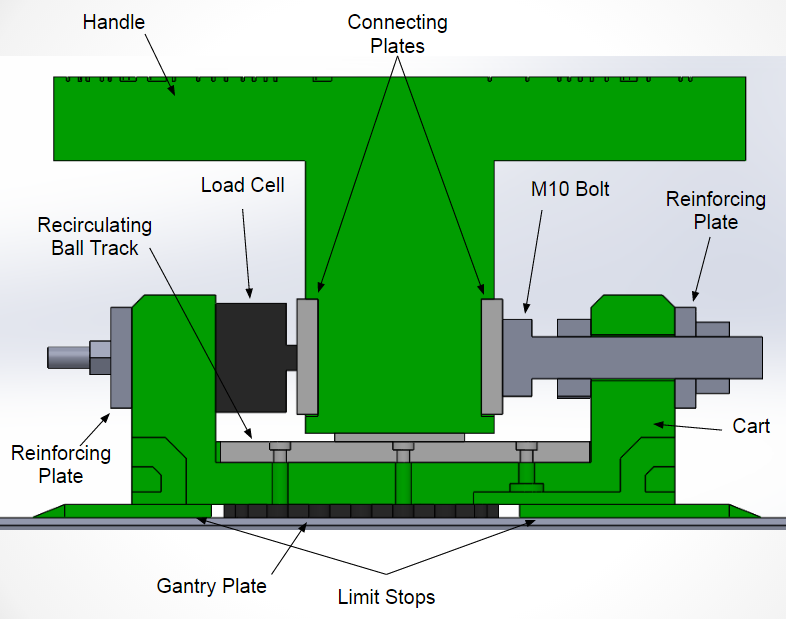
\includegraphics[width=1\columnwidth]{Images/Ball_Track_Cross_Section}
\caption{Cart Cross Section}
\label{fig:Ball_Track_Cross_Section}
\end{figure}

\begin{figure}[H]
	\centering
	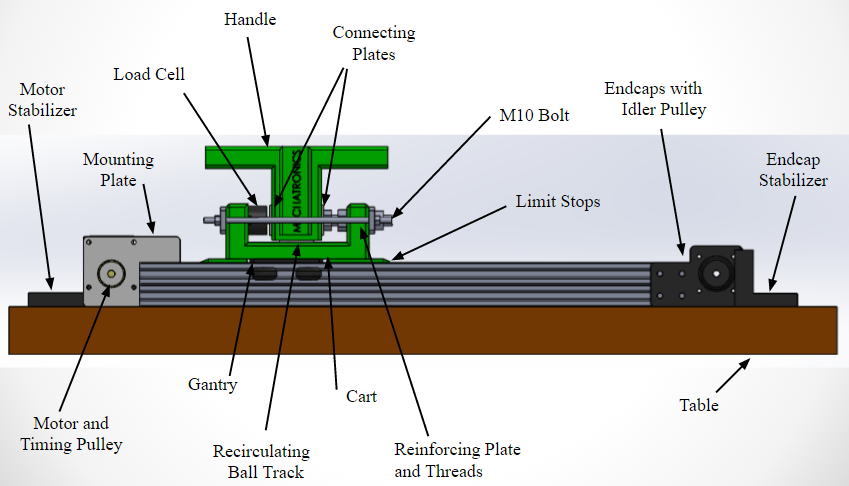
\includegraphics[width=1\linewidth]{Images/Annotated_Front}
	\caption{Front View}
	\label{fig:Annotated_Front}
\end{figure}
When designing the cart, PLA creep stiffness was not taken into account. Due to the rather elastic PLA material, a constant decrease in the preload would occur. This caused inconsistent force readings from the load cell. To counter this problem, two aluminum reinforcing plates were machined and held by threaded rods shown in Figure \ref{fig:Annotated_Iso}. This helped with the creep and overall cart stiffness, which gave much more accurate force readings from the load cell.

\begin{figure}[H]	
\centering
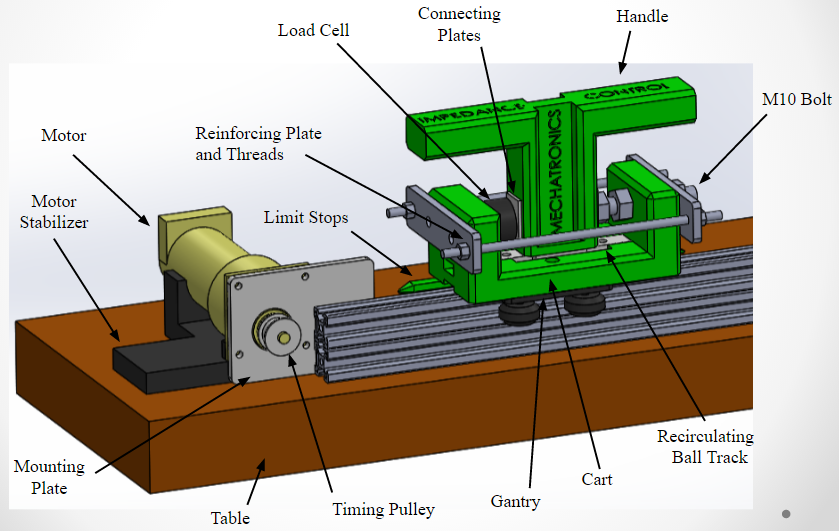
\includegraphics[width=1\linewidth]{Images/Annotated_Iso}
\caption{Detailed Isometric View}
\label{fig:Annotated_Iso}
\end{figure}

The cart and handle were 3D printed because it allowed for quick changes and variation to the design. After encountering the PLA creep problem, a future improvement would be to make the cart and handle out of aluminum. Even though that would increase costs, material, and the complexity of the design, that would ultimately eliminate any kind of creeping and preloading inconsistencies. 
\subsubsection*{ --- Electrical}
\subsubsection*{ --- Computational}
The closed loop continuous time transfer function of the complete system was 
\begin{equation}
v_{act}=\frac{s^{2}}{s^{2}+\frac{K_{P}K_{A}K_{M}N}{r(M+\frac{JN^{2}}{r^{2}})}s+\frac{K_{I}K_{A}K_{M}N}{r(M+\frac{JN^{2}}{r^{2}})}}
\end{equation}
which is second order. This fact allowed us to find the controller gains analytically from specific relations between the damping ratio and natural frequency of a second order system and its overshoot and settling time, respectively. The damping ratio can be related to the overshoot by
\begin{equation}
\zeta=|\frac{\ln{\frac{OS}{100}}}{\sqrt{\pi^{2}+(ln{\frac{OS}{100}})^{2}}}|
\end{equation}
Where
\begin{equation}
OS=Percent Overshoot
\end{equation}
The natural frequency can be related to the settling time by
\begin{equation}
\omega_{n}=\frac{4}{\zeta T_{s}}
\end{equation}
Solving for $ K_{I} and K_{P} $ gives
\begin{equation}
K_{I}=\frac{\omega_{n}^{2}r(M+\frac{JN^{2}}{r^{2}})}{K_{A}K_{M}N}
\end{equation}
\begin{equation}
K_{P}=\frac{2\omega_{n}\zeta r(M+\frac{JN^{2}}{r^{2}})}{K_{A}K_{M}N}
\end{equation}
With these gains, we used MATLAB's "c2d" built-in function to develop a biquad cascade of the discrete time transfer function of the controller utilizing Tustin's approximation. This was written to a header file for C that could be used in the final program.
In addition to finding the appropriate control gains and implementing them through a biquad cascade, we needed to also develop a biquad cascade, by hand, for computing the response of the reference system to the human input force. MATLAB was not used because we wanted a symbolic relationship between the coefficients of the biquad and the reference system parameters in order to enable the user to update the mass, spring and damping while the program was running. The reference system's continuous time transfer function was
\begin{equation}
\frac{v_{ref}}{F}=\frac{s}{M_{ref}s^{2}+B_{ref}s+K_{ref}}
\end{equation}
To compute Tustin's approximation for a discrete time transfer function, a substitution for s can be made
\begin{equation}
s=\frac{2(1-z^{-1})}{T(1+z^{-1})}
\end{equation}
Where
\begin{equation}
T= sample\ period
\end{equation}
The result is a discrete time transfer function of the form
\begin{equation}
H(z)=\frac{b_{0}+b_{1}z^{-1}+b_{2}z^{-2}}{a_{0}+a_{1}z^{-1}+a_{2}z^{-2}}
\end{equation}
For our system, the coefficients were
\begin{eqnarray}
b_{0}=\alpha \\
b_{1}=0 \\
b_{2}=-\alpha \\
a_{0}=1 \\
a_{1}=\alpha(-K_{ref}-\frac{4M_{ref}}{T}) \\
a_{2}=\alpha(\frac2M_{ref}{T}-B_{ref}+\frac{K_{ref}T}{2})
\end{eqnarray}
Where
\begin{equation}
\alpha=(\frac{2M_{ref}}{T}+B_{ref}+\frac{K_{ref}T}{2})^{-1}
\end{equation}
The C program updates the coefficients in the biquad based on the user input every 5 milliseconds and then uses the force reading calculated from the load cell voltage as the input to a function cascade() that computes the velocity of the idealized reference system. The C program also calculates the speed of the motor from the optical encoder readings, from which it can determine the speed of the cart for comparison. The cascade() function is called once more to implement the controller and determine the control voltage to be sent to the amplifier. 
\subsubsection*{ --- Hardware}
A lot of equipment was used to complete our design. A National Instruments MyRIO was the microcomputer we used, which runs Linux and features a Field Programmable Gate Array (FPGA). The MyRIO has 4 connectors, designated A through D. On one of these connections is an LCD screen and keypad that is used for the user input and some data tracking while the program runs. On another of the MyRIO connections is a Quanser Terminal Board, a device that allows direct connection of two 5 pin DIN and 4 BNC type cables. The DIN inputs are for encoders and the BNC connectors are for Digital to Analog and Analog to Digital converters (DAC and ADC, respectively). The DAC is connected to a 24 V current amplifier with a maximum current of 4.8 A. The output of the amplifier goes directly to a Pittman 9236 brushed DC motor with an E30 series 512 pulse optical encoder and 5.9:1 gearbox. The encoder is connected to the 0th encoder input on the Quanser board. The motor is mounted to an Open Builds Part Store 1.5 m V-slot belt-driven linear actuator. Mounted onto the ends of the track are two Open Build Part Store micro limit switches. The limit switches are wired through a reset switch and two mechanical relays and back into the amplifier. On the cart is a TE Connectivity Measurement Specialties FC22 Compression Load Cell. The load cell is powered by an HP signal generator at 5 V. The output of the load cell runs to the 0th ADC connector on the Quanser board as well as an oscilloscope. 
\subsubsection*{ --- Software}
Much of the software for the system was a modification from the previous quarter's embedded computing labs. The C-Code basically implements a closed-loop control system for a DC motor with a virtual reference model. The system controls the motor speed by comparing the actual velocity of the motor with the desired reference velocity. This is done through three threads: the main program thread, timer thread, and the table update thread.

The main thread accomplishes all the initialization and configuration such as the ctable structure, IRQ channel, load cell, and encoder interface. Two threads are created using \verb|pthread_create()| which start the routines \verb|Timer_Irq_Thread()| and \verb|Table_Update_Thread()|. After the initializations, it runs the table editor by calling \verb|ctable()| which runs continuously until the backspace button is entered in the keypad. When \verb|ctable()| ends, the two threads are terminated, timer IRQ is unregistered, and the MyRIO session ends.

The \verb|Timer_Irq_Thread()| schedules the next interrupt using \verb|NiFpga_WriteU32()| to write the interval time into register using the timeout value of 5000 microseconds. The timeout value is defined by the BTI value from the ctable structure. \verb|NiFpga_WriteBool()| is called to set the time register flag to true. When the interrupt is signaled, the service routine does a few things. First it calibrates the load cell by reading the analog input of the load cell voltage 10,000 times. Then the average is taken to use for the initial load cell voltage. Force reading is calculated by taking the difference of the input load cell voltage and the initial load cell voltage, then multiplying by 124.1897 which is determined from experimental data. A deadband is implemented to reject any voltage reading under 1 Newton. This will ensure the cart stays stationary when there is no input force and help eliminate noise to the load cell.

Next the reference system is calculated using the biquad cascade and Tustin's approximation explained in the Computational section. If the control voltage reaches the limit voltage, it will set \verb|VLimitFlag| which will cut off the force input into the reference system. This will slow down the reference system will slow down and the physical cart will be able to catch up. \verb|cascade()| is used to calculate the reference velocity which will be used to compare to the actual velocity. \verb|vel()| is used to measure the actual velocity of the motor which is calculated by reading the encoder counts. \verb|cascade()| calculates the control voltage using the PI controller and error between the actual and reference velocity. There is an if-statement that checks for output voltage limitation and will only output the maximum and minimum values as well as warning noises to ensure safety. Then \verb|Aio_Write()| is used to send the control voltage to the DAC. After each iteration, the interrupt service is acknowledged with \verb|Irq_Acknowledge|. The thread will terminate when signaled.

The \verb|Table_Update_Thread()| has no interrupt and is only terminated by the ready flag. It periodically calls \verb|update()| which refreshes the LCD screen display values. The timing of the update is based on \verb|nanosleep()| which waits for imprecisely 0.5 seconds. 
\subsubsection*{ --- Integration}   

%---Prototype
\subsection*{Prototype}
\subsubsection*{ --- Purpose}
The purpose of the prototype was to verify that the controller design would accomplish the goals set at the inception of the project. Constructing the prototype and running several tests ranging from simulated forces (voltage values set in the program in place of load cell voltage readings) to constant force inputs to random force inputs. Data was collected for the force input and velocity output and compared to Simulink results for the same system. Comparing the results and determining the true overshoot and settling times of the response allows quantification of the effectiveness of the controller and modeling.
\subsubsection*{ --- Description \& Implementation}
\subsubsection*{ --- Testing Results}
Two methods are used to test and validate system's performance. First, an arbitrary force is applied to the handle, after user terminates the program, both force readings and velocities are exported to MATLAB file for validation. In this case, input mode 1, which uses actual reading as force input for Simulink model, is used. A sample plot of the simulated results vs. actual velocity can be found in Figure \ref{fig:ArbitraryInput} in Appendix. Error between recorded and reference speed is also calculated by taking average of error at each time stamp and it is found to be in the scale of $10^{-6}$. 

The second method utilizes a pulley and weight system. The mechanism simulates a constant force input on the handle. Same weight is used in all tests to keep input force a constant. Equivalent force applied on the handle is approximately 3N. The 3N force is also used in simulation as a step input. Three sets of tests are run using this method and each set contains three cases. In each set, only one virtual parameter is adjusted. 

As shown in Figure \ref{fig:MChange}, spring constant is eliminated for clarity of the test, damping is kept at a constant of 50 N*s/m and mass ranges from 5kg to 40kg. In each plot, green lines represent the actual velocity recorded by C, red and blue lines represent reference velocity calculated by C and Simulink respectively. From left to right, mass is 5kg, 20kg and 40kg for each line. The lines represent different acceleration due to change in mass.  Since all three cases utilize the same input force and damping constant, their steady state speed all converge to the same point which is expected from $F=B*v$.
\begin{figure}[H]
\centering
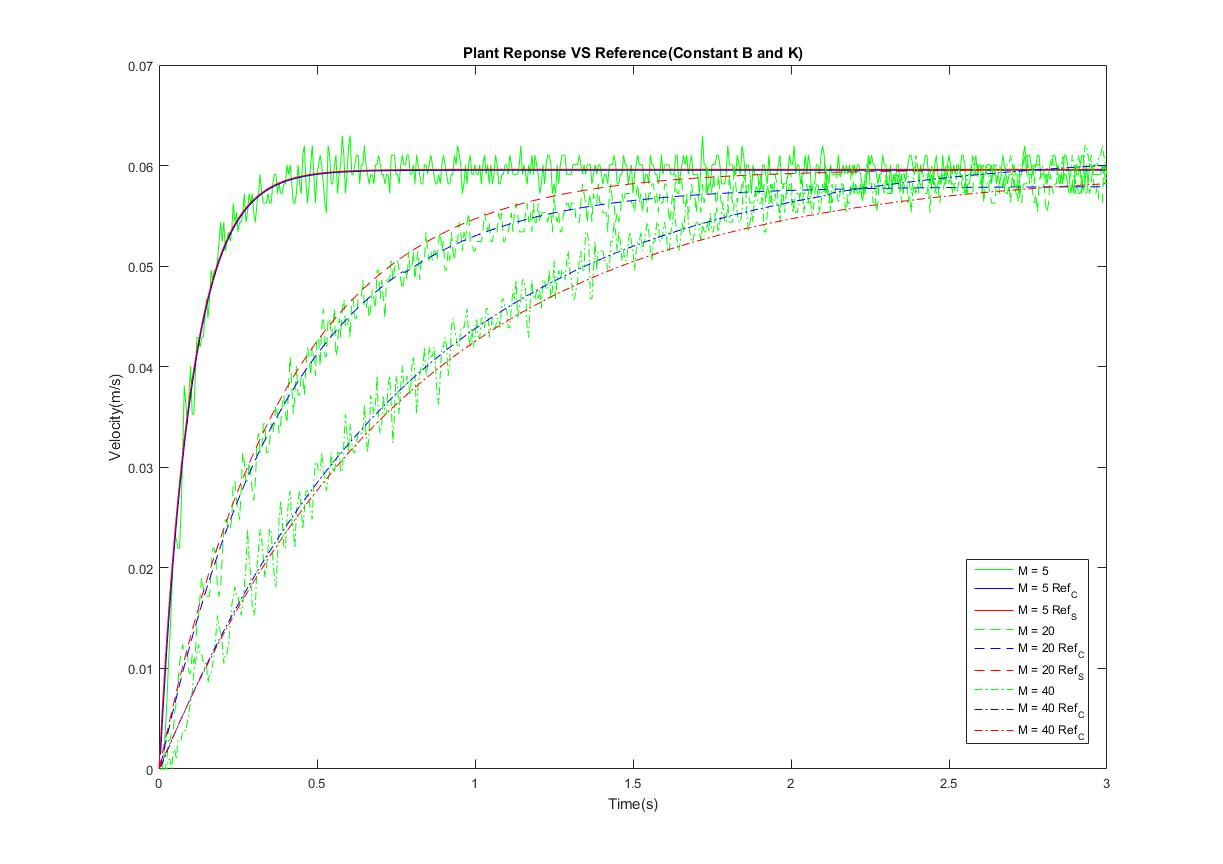
\includegraphics[width=1\linewidth]{Images/MChange}
\caption{Actual and Reference Velocity for Constant Damping with Adjusted Mass System}
\label{fig:MChange}
\end{figure}

Shown in Figure \ref{fig:BChange} is a same virtual mass with different damping constants applied on it. For all cases, mass is kept at 10kg whereas damping ranges from 25N*s/m to 100N*s/m. The steady state speed now changes due to the change in damping constant, which can be verified using equation mentioned in previous paragraph. From top to bottom, damping constant is 25N*s/m, 50 N*s/m and 100N*s/m for each case. 
\begin{figure}
\centering
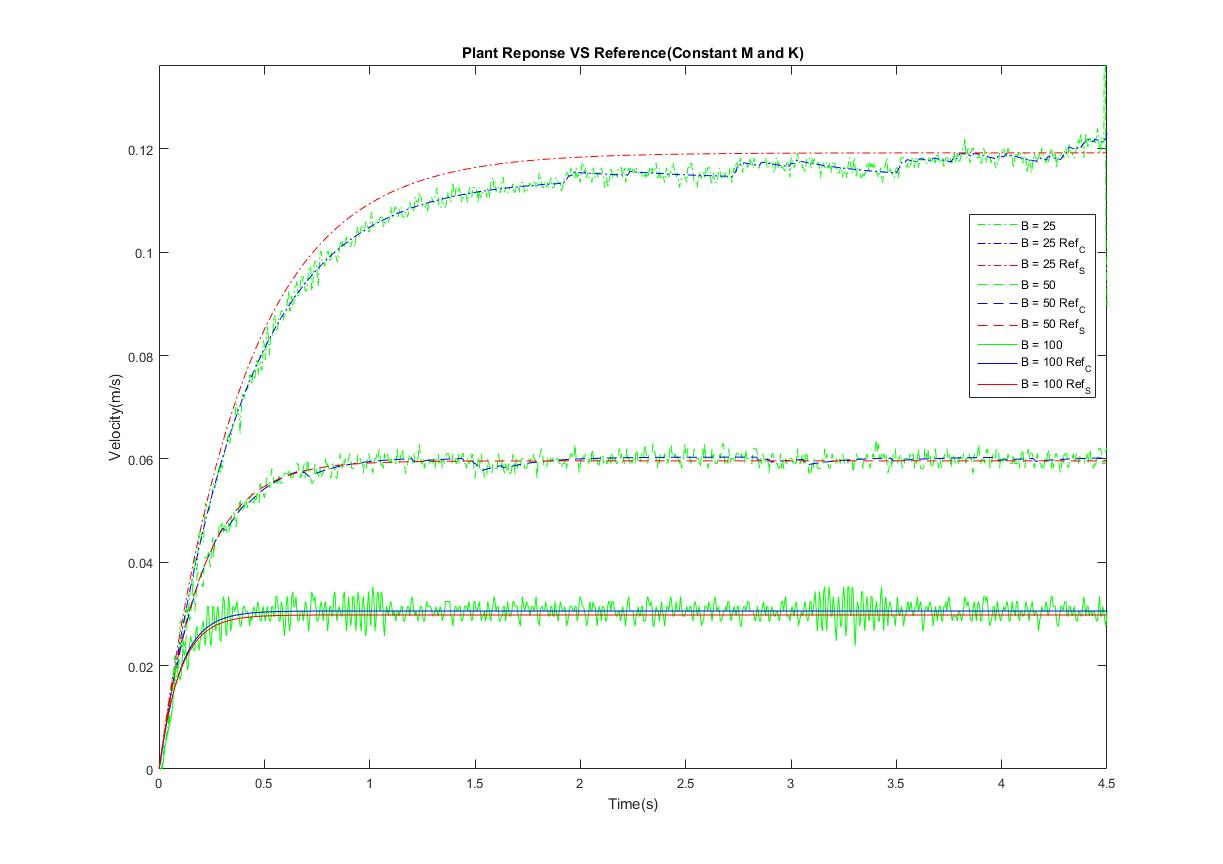
\includegraphics[width=1\linewidth]{Images/BChange}
\caption{Actual and Reference Velocity for Constant Mass with Adjusted Damping System}
\label{fig:BChange}
\end{figure}

Lastly, shown in Figure \ref{fig:KChange}, both mass and damping are kept constant and spring is the only variable. From top to bottom, spring constant increases from 0 to 20N/m. The change in spring constant resulted in a different deceleration rate for the systems. 
\begin{figure}[H]
\centering
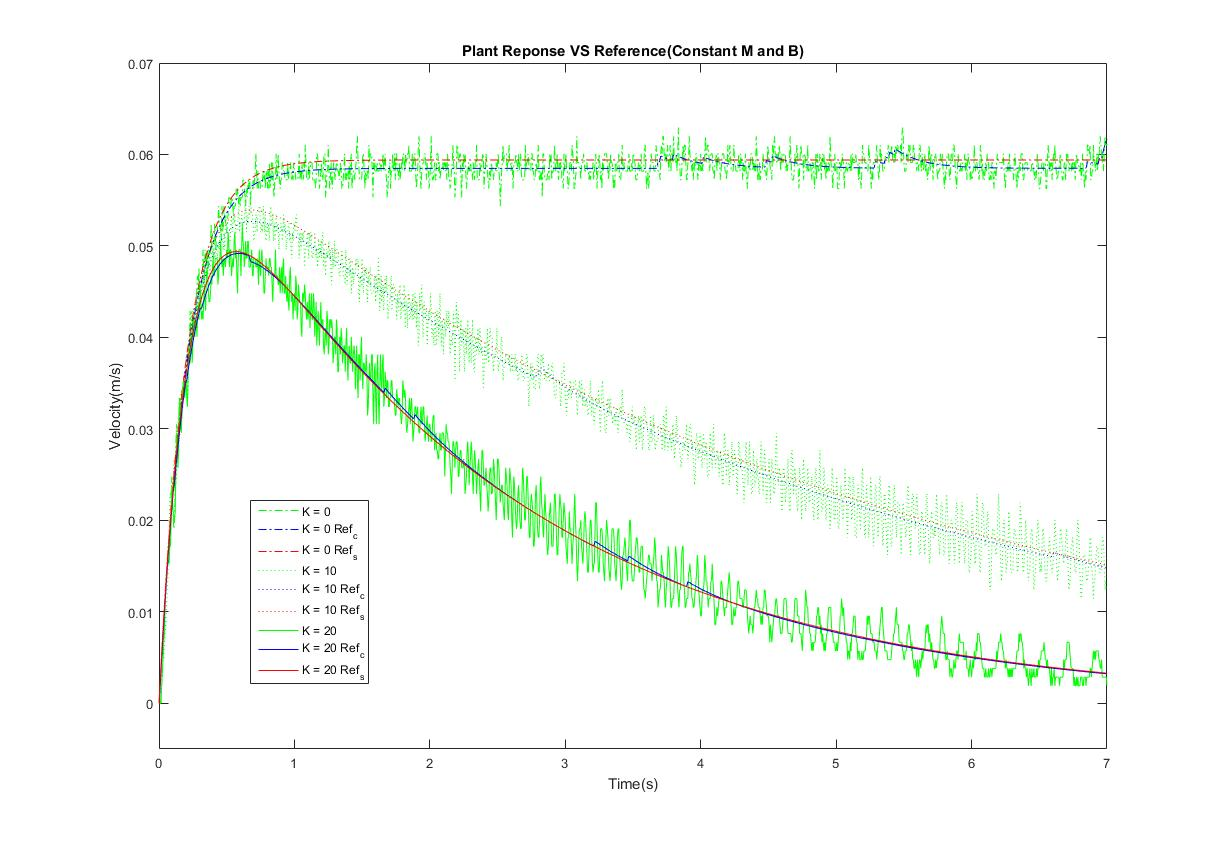
\includegraphics[width=1\linewidth]{Images/KChange}
\caption{Actual and Reference Velocity for Constant Mass and Damping with Adjusted Spring System}
\label{fig:KChange}
\end{figure}

In all three sets, there are significant amount of spikes in recorded velocity, this is mainly due to the small range of speed these tests run at. Since all deviations in speed are on the scale of $10^-3$m/s range, they won't affect overall response. The system is also tested near boundary conditions. The controller is able to handle listed force input for larger force inputs. For smaller force inputs, the noise from load cell and vibration has a stronger effect on reference system which has more potential to cause irregular activity for the motor. Both cases could easily reach the system limit as well thus triggering the warning sound.

After calculating speed error and comparing actual vs. reference response, the controller is determined to be valid and satisfy the design objectives.


%---Risk and Liability

\subsection*{Risk and Liability{{\color{red}\ *}}}
The prototype for this project and its implicated future applications carry inherent risk due to the human interaction with moving parts and machinery. While the ultimate goal of this research is to enhance the interaction between humans and machines, one or both of them may fail during operation.

Specifically for the lab prototype there are certain fail-safes implemented to prevent injury. While not as large scale as some potential industrial and commercial applications, there is still risk to the user. The track, with the motor moving the belt and cart at potentially high velocities presents a pinching or collision hazard. Although the user's hand shouldn't be near the belt during operation, should such an event occur there is a switch box with an emergency stop button connected to the amplifier that can be pressed and will cut all power to the motor immediately. Through the switch box there also runs a set of limit switches that sit at the ends of the track. These prevent the cart from running off the end of the track or into the motor. If the user inputs a force that exceeds the limits of the system, a beeping noise will be triggered through the myRIO as a warning to lower or completely remove the input. Once the force input is back in the allowable range the beeping stops and the program is ready to continue.

The future industrial and commercial uses for this type of impedance control have more risk than the prototype. Implementation in a warehouse or factory will undoubtedly introduce more axes of motion. The use of more axes requires the user to be more aware of their surroundings as items are moved around. Care must also be taken when inputting parameters to ensure correct values are being used. Incorrect values may cause the system to not work and cause damage to the machine or human. If the system fails while lifting a heavy mass, the user will be unable to move or stop the mass, potentially endangering the user, bystanders, or the environment.

%---Ethical Issues
\subsection*{Ethical Issues{{\color{red}\ *}}}
asdflkasdfasdf
%---Impact on Society
%---Impact on Society
%Help Aging population get back to work, safe working conditions, rehabilitation
\subsection*{Impact on Society} \par
Impedance control systems are utilized in many different forms all around the world to improve people's lives, from helping senior citizens getting back into the workforce to physical rehabilitation.\par
In countries such as Japan and Singapore, where the aging population are straining the country's workforce, people have been looking into technologies which can help the senior citizens go back to work again. To do that, they came up with solutions which implemented impedance control methods such as motor-assisted pallet trucks and motor-assisted exosuits so as to help the seniors push and carry heavier loads and be on par with their younger counterparts. Moreover, these solutions can also be used by their younger counterparts to reduce strain on their body and create a safer working condition for everyone.\par
For many who had suffered injury to their arm, stroke, or spinal cord, they need to undergo rehabilitation treatment in order to regain full function and control of their arm again. By using a robot with a position-based impedance controller, the therapist will be able to ask the robot to assist or resist movement of the user's wrist, elbow, or shoulder in order to simulate arm movement conditions in daily life \cite{IEEE2006}.
%---Impact on the Environment
\subsection*{Impact on the Environment{{\color{red}\ *}}}
%---Cost and Engineering Economics
\subsection*{Cost and Engineering Economics{{\color{red}\ *}}}

\begin{tabular}
	{|l|l|}
	\hline 	
	\multicolumn{2}{c}{Cost Analysis}\\ \hline
	\hline Load Cell & \$66.88 \\ 
	\hline V-Slot Track Setup & \$108.64 \\ 
	\hline Pittman Motor & \$318.00 \\ 
	\hline MyRIO & \$1000.00 \\ 
	\hline Switch Box + Relays & \$35.44 \\ 
	\hline PLA Filament & \$50.00 \\ 
	\hline All Fasteners & \$7.36 \\ \hline
	\hline Total Project Value & \$1584.67 \\ 
	\hline 
\end{tabular} 


%---Codes and Standards
\subsection*{Codes and Standards{{\color{red}\ *}}}
In the design and assembly of the prototype, we soldered together several different components. To avoid damage to the components and ensure proper functionality, the soldering had to be done according to certain standards. For example, the encoder has four leads bundled into one cable. Each lead was separately soldered to the appropriate pin on the DIN including shrink wrapping each individual wire as well as the complete bundle. The shrink wrapping is important to ensure no wires are crossed which could result in damage to one or more components. 

%---Conclusions
\subsection*{Conclusions{\color{red}\ *}}
\subsubsection*{ --- Continued Development}
\subsubsection*{ --- Final Product Configuration}

%---Bibliography
\subsection*{Bibliograph}
-- Books, Articles, Data Sheets, etc., Cited in the body. 

See the \verb|.tex| file for the commands that build the following bibliography using \BibTeX. Examples of applications that can be used to manage the \BibTeX\  file include \verb|JabRef| (windows) and \verb|BibDesk| (os x).
\bibliographystyle{plain}		% (uses file "plain.bst")
\bibliography{Mechatronics}	% expects file "Mechatronics.bib"


%---Appendices
\subsection*{Appendices{\color{red}\ *}}
\subsubsection*{ --- Drawings}
\begin{enumerate}
\item{Mechanical}
\item{Electrical (individual components and connections)}
\item{Computer Hardware}
\item{Software Descriptions (flow charts, hierarchical diagrams, etc.)}
\end{enumerate}

\subsubsection*{ --- Code}
\begin{enumerate}
\item{MATLAB analysis and design}   {\color{red}\bf{*}}
\item{C-Code} {\color{red}\bf{*}}
\end{enumerate}
\subsubsection*{ --- Major components list for prototype}
\begin{enumerate}
\item{Manufacturer}
\item{Model number}
\item{Cost}
\end{enumerate}

\newpage
\subsubsection*{Here are some \LaTeX\ examples.} 

Examine the \verb|.tex| file to see how these were implemented.

\vspace{.167in}
A figure, with a graphic inserted from a \verb|.pdf| file, with a reference to the figure in the text.
\begin{figure}[htbp]
\begin{center}
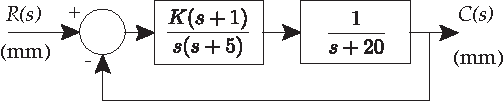
\includegraphics[width=2.75in]{ControlLoop2.pdf}
\caption{Control loop diagram}
\label{ControlLoop}
\end{center}
\end{figure}

Later on in the text: \dots We cite Figure \ref{ControlLoop} above.  Note the use of the \verb|\label{}| and \verb|\ref{}|.

Here are some numbered equations, with a reference.
\begin{equation}
T(s)=\frac{C(s)}{R(s)}=\frac{G(s)}{1+G(s)H(s)}
\label{eTF}
\end{equation}
\begin{equation}
\ket{f(x)} = \frac{1}{\sqrt{r}}\sum_{\ell=0}^{r-1}e^{2\pi i \ell/r}\ket{\hat{f}(\ell)}
\label{eFT}
\end{equation}

Elsewhere in  the text the equations \ref{eTF} and \ref{eFT} are cited. Note the use of the \verb|\label{}| and \verb|\ref{}|.

\vspace{.167in}
Here is an inline equation $f(t)=m\dot{v}(t)$. 
 
\vspace{.167in}
Some citations \cite{Bendat1971}, \cite{PhysRev.104.563}, \cite{Oppenheim1975}, and \cite{Papoulis1965}. 
 
\vspace{.167in}
A good \LaTeX\ reference is \cite{Lamport1994}.  See References.

\vspace{.167in}
The \verb|tabular| environment is tricky. 

But, it produces nice tables!

\vspace{.167in}
\begin{tabular}{|r||r@{--}l|p{1.25in}|}
\hline
\multicolumn{4}{|c|}{GG\&A Hoofed Stock}  \\  \hline  \hline
&\multicolumn{2}{c|}{Price}& \\ \cline{2-3}
\multicolumn{1}{|c||}{Year}
& \multicolumn{1}{r@{\,\vline\,}}{low}
& high & \multicolumn{1}{c|}{Comments} \\ \hline
1971 & 97 & 245 & Bad year. \\ \hline
72 & 245 &  245 & Light trading due to a heavy winter.  \\ \hline
73 & 245 & 2001 & No news was very good news this year. \\ \hline
\end{tabular}

\vspace{.5in}


\end{document}	%  <--- Here is where the document ends
